% =====================================================================================
% Manuscript (made from GubioGL/paper-template). Figures are written by run/*.py into
% paper/figures/ through src/paths.py::save_figure. Numbers come from data/resultados/.
%
% Journal class: replace the \documentclass line, for example
%   APS (PRA, PRL, ...): \documentclass[aps,pra,twocolumn,superscriptaddress,10pt]{revtex4-2}
%                        (put \maketitle after the abstract, use \affiliation, drop \date)
% =====================================================================================
\documentclass[11pt]{article}

\usepackage[margin=2.5cm]{geometry}
\usepackage{graphicx}
\usepackage{amsmath,amssymb}
\usepackage{bm}
\usepackage{booktabs}
\usepackage{xcolor}
\usepackage[numbers,sort&compress]{natbib}
\usepackage{hyperref}

\hypersetup{colorlinks=true, linkcolor=blue!50!black, citecolor=blue!50!black, urlcolor=blue!50!black}
\graphicspath{{figures/}}              % figures written by run/*.py land in paper/figures/

% Working notes: \showtodostrue -> \showtodosfalse hides every \TODO
\newif\ifshowtodos \showtodostrue
\newcommand{\TODO}[1]{\ifshowtodos\textcolor{red}{\textbf{[TODO:} #1\textbf{]}}\fi}

\title{Recovering a time-dependent control field from qubit expectation values:\\
physics-informed neural networks versus classical inversion}
\author{Gubio G. de Lima\thanks{\TODO{affiliation}. E-mail: \texttt{gubio.gomes@estudante.ufscar.br}}}
\date{\today}

\begin{document}
\maketitle

\begin{abstract}
We study the inverse problem of recovering an unknown time-dependent control field $f(t)$ of a
driven qubit, $H=\tfrac12\sigma_z+\tfrac12 f(t)\sigma_x$, from measured expectation values, and compare
physics-informed neural networks (PINNs) with classical inversion under a single protocol: identical
data, initial state $|0\rangle$, no access to the true field, five seeds, and two metrics (field error
and re-simulated trajectory error). PINNs trained with Adam alone, as in common practice, converge to
an over-smoothed field with $\sim\!25\%$ error regardless of how the field is parametrized (neural
network, Fourier series, B-splines, MixFunn). A Levenberg--Marquardt stage reduces the error by two
orders of magnitude (to $\sim\!0.2\%$), which shows that the optimizer, not the representation, is the
bottleneck. With complete, noiseless measurements, classical linear least squares and shooting with a
suitable basis remain about ten times more accurate and thousands of times faster
\TODO{update with the complete benchmark and the noisy case}. We also show why the initial
state $|+\rangle$, an eigenstate of the control operator, makes the field unidentifiable at early
times.
\end{abstract}

% -------------------------------------------------------------------------------------
\section{Introduction}\label{sec:intro}
Physics-informed neural networks (PINNs)~\cite{raissi2019pinn} have been used for quantum
control~\cite{norambuena2024pinnqc} and for learning time-independent Hamiltonian
parameters~\cite{liu2025ipinnhl}. Here we study the inverse problem of recovering an unknown
\emph{time-dependent} control field from the measured expectation values of a driven qubit, and we
ask a simple question: under a single, fair protocol, when do PINNs beat classical inversion?
Recovering a control field from measurements is relevant for calibrating and characterizing
quantum devices, where the pulse that actually reaches the qubit differs from the programmed one
\TODO{add references on pulse characterization}. Earlier PINN studies of this kind of problem
compare a single model against the ground truth. Here we compare several field parametrizations and
optimizers against classical estimators that use the same data. Section~\ref{sec:problem} states the
problem and analyses its identifiability, Sec.~\ref{sec:methods} describes the methods and the
protocol, Sec.~\ref{sec:results} presents the results, and Sec.~\ref{sec:conclusions} concludes.

Contributions:
\begin{itemize}
  \item a single protocol (same data, same initial state, no access to the true field, 5 seeds,
        two metrics) that compares four field parametrizations---neural network, periodic Fourier
        series, cosine series and B-splines, plus MixFunn~\cite{farias2025mixfunn}---and classical
        inversion (direct, linear least squares, shooting);
  \item an identifiability analysis that explains why the choice of initial state matters
        (Sec.~\ref{sec:identifiability});
  \item evidence that the optimizer, not the parametrization, limits PINN accuracy here: a
        Levenberg--Marquardt (Gauss--Newton) stage improves the field error by one to two orders of
        magnitude over Adam, in line with recent work on second-order PINN
        training~\cite{rathore2024challenges,urban2025unveiling,kiyani2025optimizer,muller2023engd,jnini2024gnngd};
  \item a spectral-resolution study: the error as a function of the frequency of the field \TODO{run}.
\end{itemize}

% -------------------------------------------------------------------------------------
\section{Problem}\label{sec:problem}
The qubit evolves under
\begin{equation}
  H(t) = \tfrac12\,\sigma_z + \tfrac12\, f(t)\,\sigma_x ,
\end{equation}
and the Bloch vector $\bm r = (X,Y,Z) = (\langle\sigma_x\rangle,\langle\sigma_y\rangle,\langle\sigma_z\rangle)$
obeys
\begin{equation}\label{eq:bloch}
  \dot X = -Y,\qquad \dot Y = X - f Z,\qquad \dot Z = f Y .
\end{equation}
Given $N=100$ equally spaced measurements of $\bm r(t_i)$ on $[0,T]$, possibly with Gaussian noise of
standard deviation $\sigma$, we want $f(t)$.
Test fields: (1) $f=\cos t$, $T=2\pi$; (2) $f = 1.5\sin 2t + 0.8\cos(3.5t+0.5) + 0.4\sin 7t$, $T=2.52\pi$;
(3) $f = [1.5\sin 2t - 0.3\cos(3t-0.5) + 0.4\sin 7t]\,\sin^2(\pi t/T)$, $T=2.52\pi$;
and, for the spectral study, single-tone pulses $f=\sin(\omega t)\sin^2(\pi t/T)$.

\subsection{Identifiability and choice of the initial state}\label{sec:identifiability}
The field enters Eq.~\eqref{eq:bloch} only through $fZ = X-\dot Y$ and $fY=\dot Z$, so the information
on $f(t)$ carried by the data is proportional to $Y^2+Z^2 = 1-X^2$. The state $|+\rangle$, an
eigenstate of the control operator $\sigma_x$, gives $Y^2+Z^2=0$ at $t=0$: there the field has no
effect on the state and cannot be identified. With $|0\rangle$, $\dot Y(0) = -f(0)$ and
$Y^2+Z^2 \geq 0.13$ over the whole interval for the three test fields (Fig.~\ref{fig:observability}).
We therefore use $|0\rangle$ throughout. With the same measurement budget this halves the error of
the classical estimators and reduces its spread across noise realizations
(from $0.15\pm0.05$ to $0.07\pm0.01$ for linear least squares at $\sigma=0.01$, five noise
realizations; \texttt{data/parte1/resultados\_desenho\_experimental.csv}). With only $\langle\sigma_z\rangle$ measured, however, $|0\rangle$ makes
$f$ and $-f$ indistinguishable, because $\sigma_z H(f)\sigma_z = H(-f)$.

\begin{figure}[t]
  \centering
  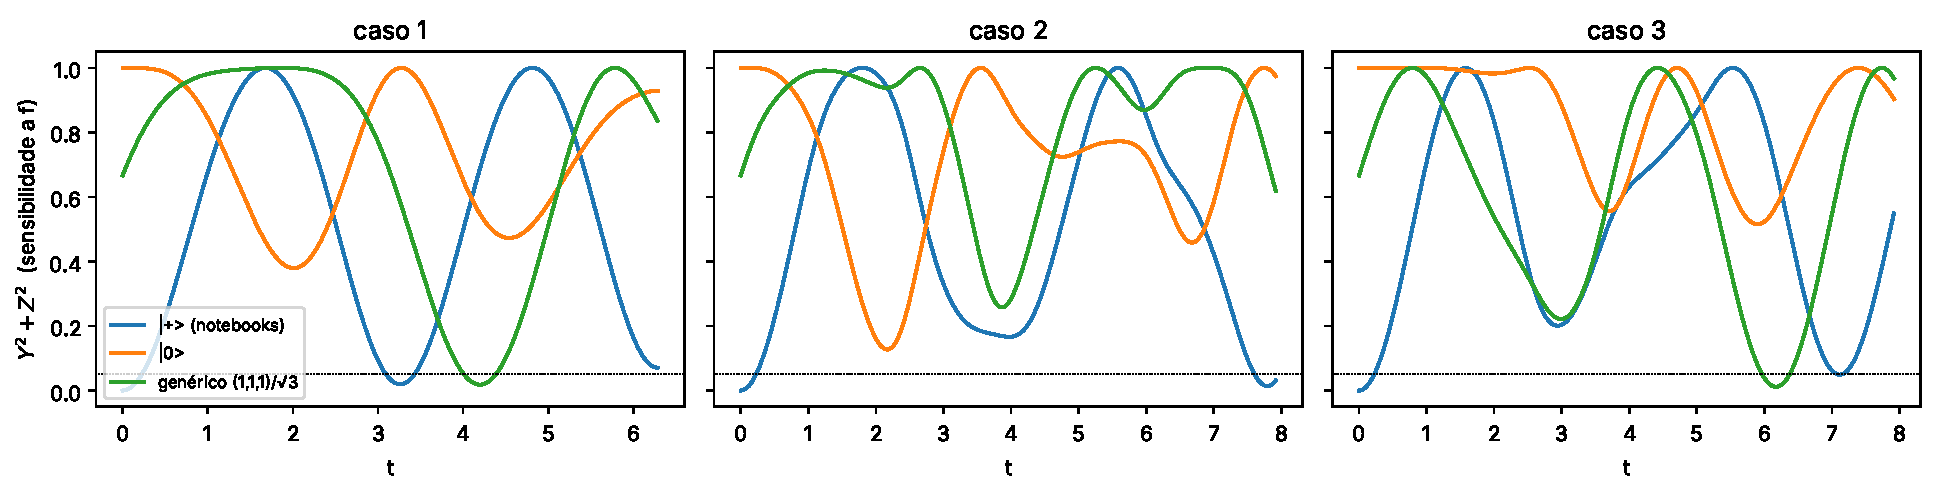
\includegraphics[width=\linewidth]{observabilidade.pdf}
  \caption{$Y^2+Z^2$, the sensitivity of the data to the field, for three initial states.
  Produced by \texttt{run/diagnostico.py}.}
  \label{fig:observability}
\end{figure}

% -------------------------------------------------------------------------------------
\section{Methods}\label{sec:methods}

\paragraph{Field parametrizations.} (i) Fourth output of the state network; (ii) periodic Fourier
series with period $T$ and $M=10$ harmonics; (iii) cosine series $\sum_{n=0}^{40} c_n\cos(n\pi t/T)$,
which has no Gibbs phenomenon when $f(0)\neq f(T)$; (iv) cubic B-splines with 80 uniform basis
functions; (v) MixFunn~\cite{farias2025mixfunn}.

\paragraph{PINN.} A network $\mathrm{NN}(s)$ with input $s=2t/T-1$ represents the state, with the
initial condition imposed exactly, $\bm r(t) = \bm r_0 + (t/T)\,\mathrm{NN}(s)$. When the pulse is
known to start and end at zero (field~3 and the spectral pulses), the field is constrained exactly
as well, $f = g - (1-\tau)g(0) - \tau g(T)$ with $\tau=t/T$ and $g$ the unconstrained
parametrization~\cite{lu2021hard}. The loss is the sum of the mean squared residual of
Eq.~\eqref{eq:bloch} over collocation points, the mean squared data misfit and, for noisy data, a
smoothness penalty $\lambda_f T^{-1}\int f''^2\,dt$. Collocation points are the data points plus 200
uniform random points redrawn at every Adam epoch. Time derivatives are computed in forward mode
inside the network. The coefficients of linear parametrizations are initialized by linear least
squares on the data.

\paragraph{Optimization.} 3000 Adam steps (cosine schedule), followed by L-BFGS, dense BFGS, or
Levenberg--Marquardt (LM) with Nielsen's damping update~\cite{nielsen1999damping}. Because the loss is
exactly $\|\bm\rho(\theta)\|^2$ for a residual vector $\bm\rho$, the LM step is a Gauss--Newton step
in the sense of~\cite{muller2023engd,jnini2024gnngd}; when parameters outnumber residuals it is solved
in residual space~\cite{jnini2025dual}. We also tested causal weights~\cite{wang2022causality},
gradient-norm loss balancing~\cite{wang2021gradient} and variable projection.

\paragraph{Classical baselines.} Direct pointwise inversion $f = [Z(X-\dot Y)+Y\dot Z]/(Y^2+Z^2)$ with
spline derivatives; linear least squares for the coefficients of a basis; and shooting:
Bloch-equation integration with sensitivities and LM on the data misfit, initialized by least squares.

\paragraph{Protocol.} Identical data for all methods per (field, noise, seed); initial state
$|0\rangle$; the true field never enters a loss or a hyper-parameter choice (regularization weights
are fixed a priori by the noise level); five seeds; two metrics: relative $L_2$ error of the field
and the RMS error of the trajectory re-simulated with the recovered field. Code:
\texttt{src/}, \texttt{run/rodar.py}.

% -------------------------------------------------------------------------------------
\section{Results}\label{sec:results}

\begin{figure}[t]
  \centering
  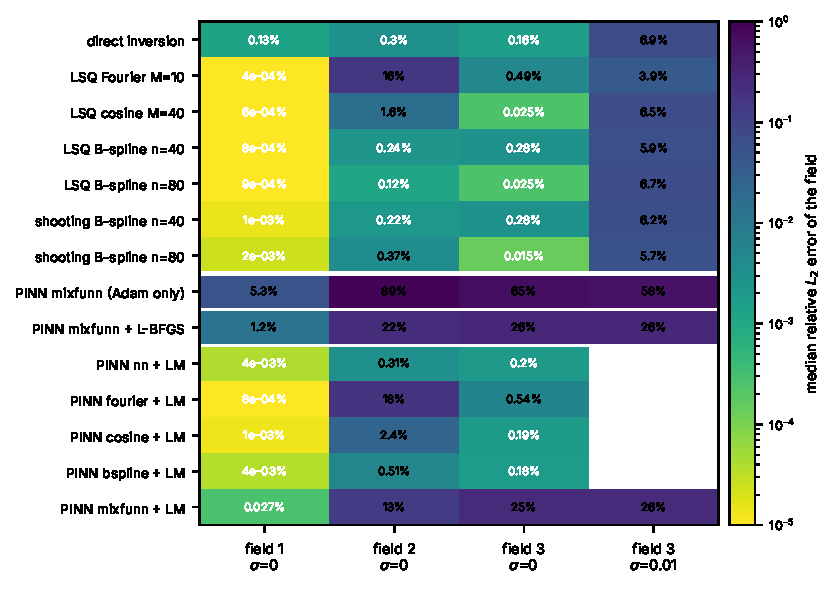
\includegraphics[width=0.8\linewidth]{fig_benchmark.pdf}
  \caption{Median relative error of the recovered field over five seeds, for every method and
  scenario (\texttt{run/fig\_artigo.py}, data in \texttt{data/resultados/padrao}).}
  \label{fig:benchmark}
\end{figure}

\TODO{Preliminary: 260 of 440 runs. Missing: PINN+LM with noise; Adam-only and L-BFGS recipes for
the network, Fourier, cosine and B-spline fields. Update every number below from
\texttt{data/resultados/padrao/RESULTADOS.md} when complete.}

\paragraph{Adam-only training.} PINNs trained as in common practice (small network, raw time input,
residual only at the data points, Adam with a fixed learning rate) recover field~3 with
$\approx 25\%$ error for every field parametrization. The recovered field is a smoothed version of the
true one, while the re-simulated trajectory is already close to the data (RMS error $\sim\!10^{-2}$):
a small trajectory error does not imply an accurate field.

\paragraph{Second-order optimization.} Adding a Levenberg--Marquardt stage after 3000 Adam steps
reduces the median field error for field~3 to $0.20\%$ (field as network output), $0.18\%$ (cubic
B-splines with 80 functions) and $0.19\%$ (cosine series), consistently over five seeds
(Fig.~\ref{fig:benchmark}). For field~1 ($\cos t$) all linear parametrizations reach
$\sim\!10^{-5}$. Once the optimizer is adequate the parametrization matters: the periodic Fourier
basis cannot represent field~2, for which $f(0)\neq f(T)$ (18\%, Gibbs phenomenon), while the
network reaches $0.31\%$. MixFunn reaches $3\times10^{-4}$ for $\cos t$, but it did not converge
within the time limit for the other fields (13--25\%).

\paragraph{Comparison with classical inversion.} With complete, noiseless measurements, classical
estimators with the same basis are more accurate than the best PINN: for field~3, shooting with
80 B-splines reaches $0.015\%$ and linear least squares $0.025\%$, against $\approx 0.2\%$ for the
PINNs, at a cost below one second instead of minutes. Enlarging the basis (40 to 80 B-splines;
cosines instead of a periodic Fourier series) improves the classical estimators by a factor of ten.
With noise ($\sigma = 0.01$) all classical estimators lie between $3.9\%$ and $6.9\%$, and the
information content of the data, not the method, limits the accuracy
\TODO{PINN results with noise}.

\begin{figure}[t]
  \centering
  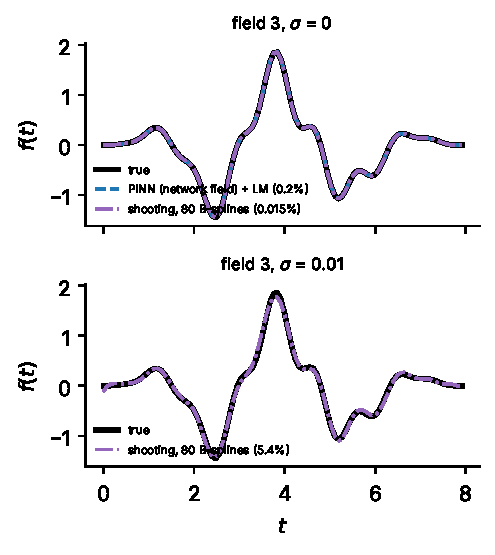
\includegraphics[width=0.6\linewidth]{fig_campos.pdf}
  \caption{Field~3 recovered by an Adam-only PINN, a PINN with an LM stage and shooting (seed 0).}
  \label{fig:fields}
\end{figure}

% Ablation figure: run `python run/rodar.py --perfil ablacao` and `python run/fig_artigo.py`
% (writes figures/fig_ablacao.pdf), then uncomment.
% \begin{figure}[t]
%   \centering
%   \includegraphics[width=0.75\linewidth]{fig_ablacao.pdf}
%   \caption{Ablation of the PINN ingredients (field~3, no noise).}
%   \label{fig:ablation}
% \end{figure}

% Spectral-resolution figure: run `python run/rodar.py --perfil espectral` and
% `python run/fig_espectral.py` (writes figures/fig_espectral.pdf), then uncomment.
% \begin{figure}[t]
%   \centering
%   \includegraphics[width=\linewidth]{fig_espectral.pdf}
%   \caption{Spectral resolution: field error versus pulse frequency $\omega$. The dotted line is the
%   highest frequency of the $M=10$ Fourier basis.}
%   \label{fig:spectral}
% \end{figure}

\TODO{Ablation (figure commented out): run profile \texttt{ablacao}. Spectral resolution: profile
\texttt{espectral} not run yet.}

% -------------------------------------------------------------------------------------
\section{Conclusions}\label{sec:conclusions}
(Preliminary.) Under a single protocol, the accuracy of PINNs for this inverse problem is limited by
the optimizer: Adam alone yields an over-smoothed field, and a Gauss--Newton (Levenberg--Marquardt)
stage improves it by two orders of magnitude. With complete, noiseless data, classical least squares
and shooting with a good basis are still more accurate and much cheaper, so the case for PINNs has to
be made where these estimators do not apply directly: partial observations (e.g.\ only
$\langle\sigma_z\rangle$, where $|0\rangle$ makes the sign of $f$ unidentifiable), several initial
states sharing one field, and open-system dynamics \TODO{}.

\bibliographystyle{unsrtnat}
\bibliography{references}

\end{document}
